\documentclass[times, utf8, seminar, numeric]{fer}
\usepackage{booktabs}
 \usepackage{url}
\usepackage{graphicx}
\usepackage{float}
\begin{document}

% Ukljuci literaturu u seminar
\nocite{*}

% TODO: Navedite naslov rada.
\title{Vlastita implementacija filtera: \protect\\ The Logarithmic Dynamic Cuckoo Filter}

% TODO: Navedite vaše ime i prezime.
\author{Fran Ostroški, Elena Wachtler}

% TODO: Navedite ime i prezime voditelja.
\voditelj{Mirjana Domazet-Lošo}

\maketitle

\tableofcontents

\chapter{Uvod}

Spomenuti glavnu temu projekta, da se radi o projektu u sklopu kolegija Bioinformatika 1. Spomenuti sve izvore iz literature, točno što je koji od njih napravio i kako se jedan razlikuje od drugog (ovo se boduje, čak 3 boda, baš se moraju spomenuti izvori u tekstu, tako piše u uputama). \\
 
Franov komentar: ako misliš da treba nešt izmijenit ili nadodat, napiši. \\

Cuckoo filtar je probabilistička struktura podataka koja se koristi za određivanje pripadnosti zadanog elementa nekom skupu. Sam filtar nastao je kao proširenje već postojećih Bloom filtara, a naziv je dobio prema ptici kukavici koja izbacuje jaja iz tuđih gnijezda kako bi ubacila svoja. \\Iako je riječ o općenitim podatcima, cuckoo filtar često se primijenjuje u bioinformatici jer je pogodna za određivanje pripadnosti podnizova nukleotidnih slijedova nekom većem nizu nukleotida ili usporedbu nalaze li se podnizovi jednog slijeda u nekom drugom slijedu.

Pripadnost elementa nekom skupu ovom strukturom ne možemo garantirati, jer zbog implementacije algoritma postoji malena šansa za "false positive" i "false negative" rezultate. Upravo zbog toga što postoji određena vjerojatnost pogreške cuckoo filtar je probabilistički. Međutim, nepripadnost nekom skupu može se pouzdano odrediti. \\

U ovom projektu u sklopu kolegija Bioinformatika 1 na Fakultetu elektrotehnike i računarstva predstavit ćemo svoju implementaciju cuckoo filtra. \\

NAPOMENA: u bibtex fileu nedostaje jedan izvor, nisam mogla naći njegov .bib: 
Fan et al. 2013. Cuckoo Filter: Better Than Bloom; https://www.cs.cmu.edu/~binfan/papers/login cuckoofilter.pdf - našla sam samo za Practically Better Than Bloom.

\chapter{Opis algoritma}
Mogu se i ovdje koristiti izvori, možda čak i bolje nego da se koriste u Uvodu, iako se mogu i u uvodu spomenuti.

\begin{flushleft}
\textbf{Vizualizacija algoritma na jednostavnom primjeru.}
\end{flushleft}


U općenitom slučaju, cuckoo filtar sastoji se nizova memorijskih lokacija koje se nazivaju \textit{bucketima}. Bucketi mogu imati mjesta za više unosa, ali u ovom jednostavnom primjeru svaki bucket moći će primiti  po 1 uneseni podatak.

Recimo da imamo jedan kratak nukleotidni slijed, npr. AACTGAT, te kao ulaze u filtar želimo unijeti sve njegove k-mere, za k = 3. To su : AAC, ACT, CTG, TGA i GAT . \\
U prvom koraku algoritma za svaki unos računaju se dva sažetka (engl. \textit{hash}) pomoću odabranih funkcija sažimanja (hash funkcija).

\begin{figure}[H]
  \centering
  \setlength{\intextsep}{5pt}
  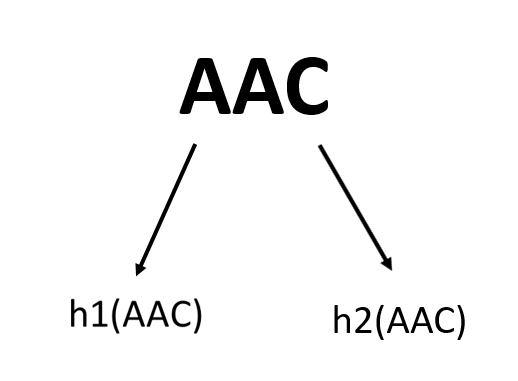
\includegraphics[scale = 0.75]{images/hashing.png}
  \caption{Generiranje hasha - Fran Ostroški}
  \label{fig_hash}
\end{figure}

U drugom koraku se iz generiranih sažetaka određuje indeks bucketa u koji će biti smješten ulazni niz. To se najčešće određuje uporabom operacije dijeljenja \textit{modulo} s ukupnim brojem bucketa. Kada se generiaju oba indeksa, element će se spremiti na jedno od dvije lokacije s tim indeksima. Svrha drugog sažetka je da bi se umanjila vjerojatnost kolizija i potreba za premještanjem. 


\begin{figure}[H]
  \centering
  \setlength{\intextsep}{5pt}
  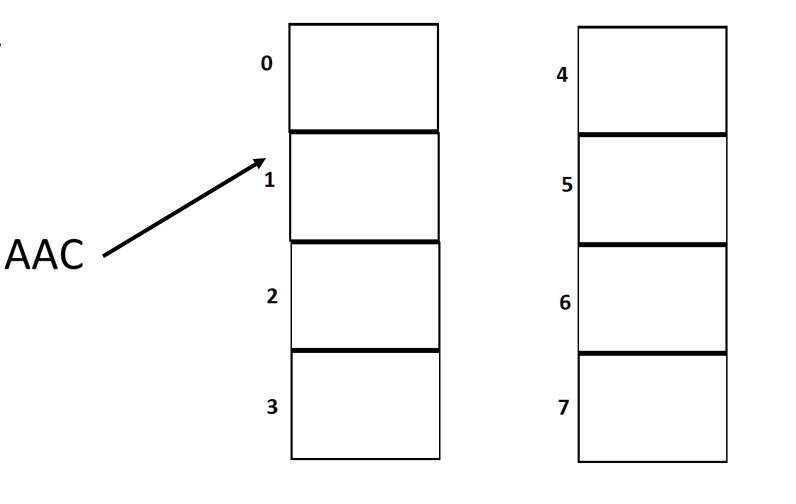
\includegraphics[scale = 0.4]{images/insertion1.png}
  \caption{Odabir lokacije za niz AAC - prikaz po uzoru na [2]}
  \label{fig_insert1}
\end{figure}
Idući na redu je niz ACT . Nakon generiranja sažetaka smješta se u prazni bucket. Budući da je bucket na jednom od dobivenih indeksa već popunjen, spremamo ga na drugo, prazno mjesto.
\begin{figure}[H]
  \centering
  \setlength{\intextsep}{5pt}
  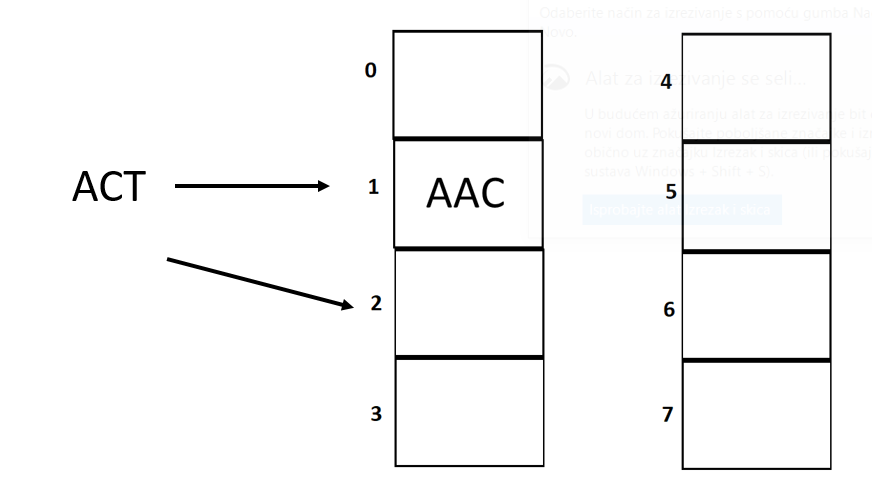
\includegraphics[scale = 0.4]{images/insertion2.png}
  \caption{Odabir lokacije za niz ACT - prikaz po uzoru na [2]}
  \label{fig_insert2}
\end{figure}

Isto korak se ponavlja za niz CTG.
\begin{figure}[H]
  \centering
  \setlength{\intextsep}{5pt}
  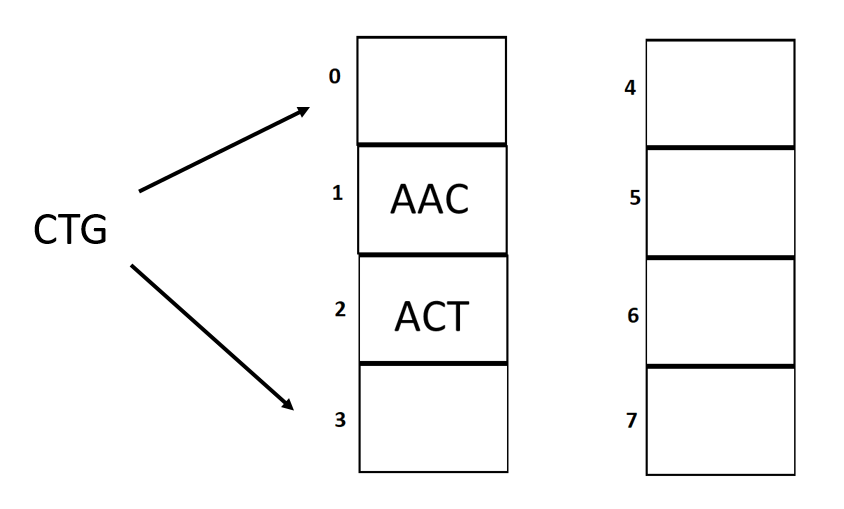
\includegraphics[scale = 0.4]{images/insertion3.png}
  \caption{Odabir lokacije za niz CTG - prikaz po uzoru na [2]}
  \label{fig_insert3}
\end{figure}

Za niz TGA dogodila se situacija da oba pokazivača pokazuju na indekse s već popunjenim bucketima. Sada se u algoritmu događa "izbacivanje". Obabrani element izbacujemo, umećemo TGA, a za izbačeni element tražimo novu lokaciju. Odabir lokacije se razlikuje od algoritma do algoritma.

\begin{figure}[H]
  \centering
  \setlength{\intextsep}{5pt}
  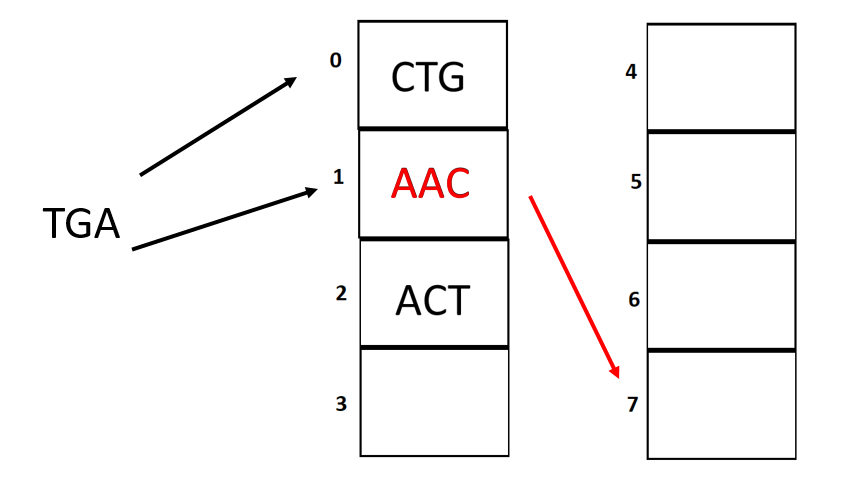
\includegraphics[scale = 0.4]{images/swap1.png}
  \caption{Izbacivanje AAC i ubacivanje TGA - prikaz po uzoru na [2]}
  \label{fig_swap1}
\end{figure}

Za niz GAC također se mora izvršiti izbacivanje starog elementa. 

\begin{figure}[H]
  \centering
  \setlength{\intextsep}{5pt}
  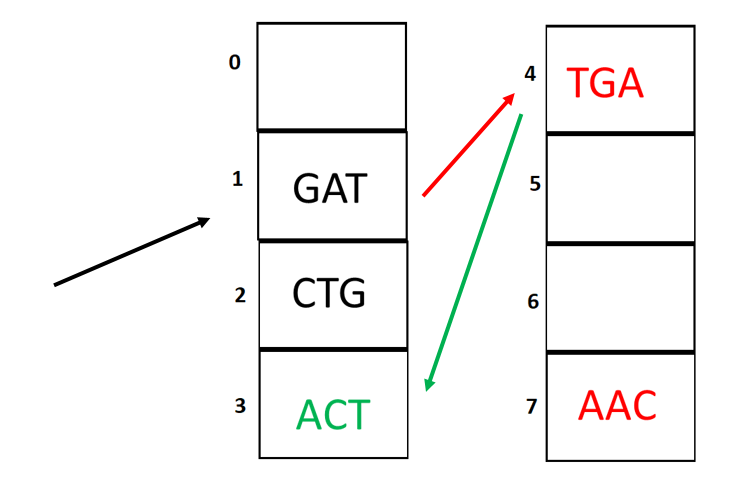
\includegraphics[scale = 0.4]{images/swap2.png}
  \caption{Izbacivanje ACT i ubacivanje GAC - prikaz po uzoru na [2]}
  \label{fig_swap2}
\end{figure}

\begin{figure}[H]
  \centering
  \setlength{\intextsep}{5pt}
  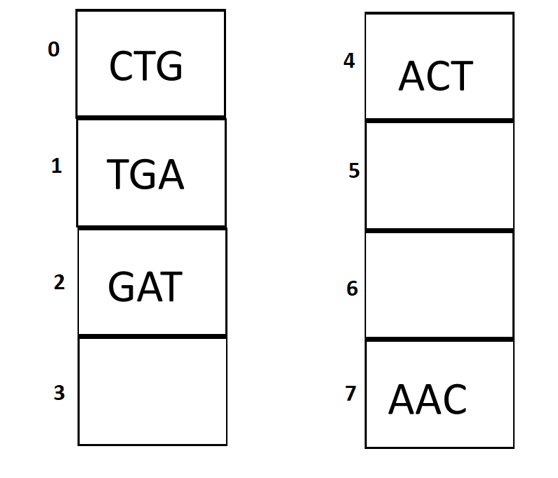
\includegraphics[scale = 0.4]{images/finalalign.png}
  \caption{Konačni razmještaj elemenata - prikaz po uzoru na [2]}
  \label{fig_finalalign}
\end{figure}

Možemo primjetiti da što je popunjenost veća raste vjerojatnost da će doći do izbacivanja i relokacije starijih elemenata u filtru. Dogodit će se situacije da će element koji relociramo biti premješten na već popunjeni bucket. U tom slučaju prijašnji element će se relocirati, i tako dalje sve dok se ne pronađe slobodno mjesto ili se dosegne maksimalan broj operacija premještanja. U slučaju da se dosegne maksimalan broj, to je obično indikator skore popunjenosti filtra. U tom slučaju mogu se poduzeti razne akcije, koje su ponovno različite za svaku implementaciju filtra. \\

NAPOMENA: Eventualno doradit opise, dodat usporedbe tih algoritama iz dokumentacije po čemu se razlikuju, ali neznam dal smijem njihove slike (npr. tablice s vremenskim složenostima i to) jer piše u uputama kao da treba dopuštenje autora. 

 
\chapter{Analiza}
Analiza točnosti, vremena izvođenja i utroška memorije za različite testne slučajeve - ovo nosi 3 boda. Testira se na stvarnim podatcima, kod nas E. coli - rezultati prikazani u tablici ili grafu.

\chapter{Zaključak}
Zaključak.

\bibliography{literatura}
\bibliographystyle{fer}

\chapter{Sažetak}
U ovome radu dan je pregled vlastite implementacije rješenja problema opisanog u znanstvenim radovima koja je napravljena u sklopu projekta iz kolegija Bioinformatika 1 na Fakultetu elektrotehnike i računarstva Sveučilišta u Zagrebu.

\end{document}
